% Options for packages loaded elsewhere
\PassOptionsToPackage{unicode}{hyperref}
\PassOptionsToPackage{hyphens}{url}
\PassOptionsToPackage{dvipsnames,svgnames,x11names}{xcolor}
%
\documentclass[
  letterpaper,
  DIV=11,
  numbers=noendperiod]{scrreprt}

\usepackage{amsmath,amssymb}
\usepackage{iftex}
\ifPDFTeX
  \usepackage[T1]{fontenc}
  \usepackage[utf8]{inputenc}
  \usepackage{textcomp} % provide euro and other symbols
\else % if luatex or xetex
  \usepackage{unicode-math}
  \defaultfontfeatures{Scale=MatchLowercase}
  \defaultfontfeatures[\rmfamily]{Ligatures=TeX,Scale=1}
\fi
\usepackage{lmodern}
\ifPDFTeX\else  
    % xetex/luatex font selection
\fi
% Use upquote if available, for straight quotes in verbatim environments
\IfFileExists{upquote.sty}{\usepackage{upquote}}{}
\IfFileExists{microtype.sty}{% use microtype if available
  \usepackage[]{microtype}
  \UseMicrotypeSet[protrusion]{basicmath} % disable protrusion for tt fonts
}{}
\makeatletter
\@ifundefined{KOMAClassName}{% if non-KOMA class
  \IfFileExists{parskip.sty}{%
    \usepackage{parskip}
  }{% else
    \setlength{\parindent}{0pt}
    \setlength{\parskip}{6pt plus 2pt minus 1pt}}
}{% if KOMA class
  \KOMAoptions{parskip=half}}
\makeatother
\usepackage{xcolor}
\setlength{\emergencystretch}{3em} % prevent overfull lines
\setcounter{secnumdepth}{5}
% Make \paragraph and \subparagraph free-standing
\ifx\paragraph\undefined\else
  \let\oldparagraph\paragraph
  \renewcommand{\paragraph}[1]{\oldparagraph{#1}\mbox{}}
\fi
\ifx\subparagraph\undefined\else
  \let\oldsubparagraph\subparagraph
  \renewcommand{\subparagraph}[1]{\oldsubparagraph{#1}\mbox{}}
\fi


\providecommand{\tightlist}{%
  \setlength{\itemsep}{0pt}\setlength{\parskip}{0pt}}\usepackage{longtable,booktabs,array}
\usepackage{calc} % for calculating minipage widths
% Correct order of tables after \paragraph or \subparagraph
\usepackage{etoolbox}
\makeatletter
\patchcmd\longtable{\par}{\if@noskipsec\mbox{}\fi\par}{}{}
\makeatother
% Allow footnotes in longtable head/foot
\IfFileExists{footnotehyper.sty}{\usepackage{footnotehyper}}{\usepackage{footnote}}
\makesavenoteenv{longtable}
\usepackage{graphicx}
\makeatletter
\def\maxwidth{\ifdim\Gin@nat@width>\linewidth\linewidth\else\Gin@nat@width\fi}
\def\maxheight{\ifdim\Gin@nat@height>\textheight\textheight\else\Gin@nat@height\fi}
\makeatother
% Scale images if necessary, so that they will not overflow the page
% margins by default, and it is still possible to overwrite the defaults
% using explicit options in \includegraphics[width, height, ...]{}
\setkeys{Gin}{width=\maxwidth,height=\maxheight,keepaspectratio}
% Set default figure placement to htbp
\makeatletter
\def\fps@figure{htbp}
\makeatother
% definitions for citeproc citations
\NewDocumentCommand\citeproctext{}{}
\NewDocumentCommand\citeproc{mm}{%
  \begingroup\def\citeproctext{#2}\cite{#1}\endgroup}
\makeatletter
 % allow citations to break across lines
 \let\@cite@ofmt\@firstofone
 % avoid brackets around text for \cite:
 \def\@biblabel#1{}
 \def\@cite#1#2{{#1\if@tempswa , #2\fi}}
\makeatother
\newlength{\cslhangindent}
\setlength{\cslhangindent}{1.5em}
\newlength{\csllabelwidth}
\setlength{\csllabelwidth}{3em}
\newenvironment{CSLReferences}[2] % #1 hanging-indent, #2 entry-spacing
 {\begin{list}{}{%
  \setlength{\itemindent}{0pt}
  \setlength{\leftmargin}{0pt}
  \setlength{\parsep}{0pt}
  % turn on hanging indent if param 1 is 1
  \ifodd #1
   \setlength{\leftmargin}{\cslhangindent}
   \setlength{\itemindent}{-1\cslhangindent}
  \fi
  % set entry spacing
  \setlength{\itemsep}{#2\baselineskip}}}
 {\end{list}}
\usepackage{calc}
\newcommand{\CSLBlock}[1]{\hfill\break\parbox[t]{\linewidth}{\strut\ignorespaces#1\strut}}
\newcommand{\CSLLeftMargin}[1]{\parbox[t]{\csllabelwidth}{\strut#1\strut}}
\newcommand{\CSLRightInline}[1]{\parbox[t]{\linewidth - \csllabelwidth}{\strut#1\strut}}
\newcommand{\CSLIndent}[1]{\hspace{\cslhangindent}#1}

\usepackage{musicography}
\KOMAoption{captions}{tableheading}
\makeatletter
\@ifpackageloaded{caption}{}{\usepackage{caption}}
\AtBeginDocument{%
\ifdefined\contentsname
  \renewcommand*\contentsname{Índice}
\else
  \newcommand\contentsname{Índice}
\fi
\ifdefined\listfigurename
  \renewcommand*\listfigurename{Lista de Figuras}
\else
  \newcommand\listfigurename{Lista de Figuras}
\fi
\ifdefined\listtablename
  \renewcommand*\listtablename{Lista de Tabelas}
\else
  \newcommand\listtablename{Lista de Tabelas}
\fi
\ifdefined\figurename
  \renewcommand*\figurename{Figura}
\else
  \newcommand\figurename{Figura}
\fi
\ifdefined\tablename
  \renewcommand*\tablename{Tabela}
\else
  \newcommand\tablename{Tabela}
\fi
}
\@ifpackageloaded{float}{}{\usepackage{float}}
\floatstyle{ruled}
\@ifundefined{c@chapter}{\newfloat{codelisting}{h}{lop}}{\newfloat{codelisting}{h}{lop}[chapter]}
\floatname{codelisting}{Listagem}
\newcommand*\listoflistings{\listof{codelisting}{Lista de Listagens}}
\makeatother
\makeatletter
\makeatother
\makeatletter
\@ifpackageloaded{caption}{}{\usepackage{caption}}
\@ifpackageloaded{subcaption}{}{\usepackage{subcaption}}
\makeatother
\ifLuaTeX
\usepackage[bidi=basic]{babel}
\else
\usepackage[bidi=default]{babel}
\fi
\babelprovide[main,import]{brazilian}
% get rid of language-specific shorthands (see #6817):
\let\LanguageShortHands\languageshorthands
\def\languageshorthands#1{}
\ifLuaTeX
  \usepackage{selnolig}  % disable illegal ligatures
\fi
\usepackage{bookmark}

\IfFileExists{xurl.sty}{\usepackage{xurl}}{} % add URL line breaks if available
\urlstyle{same} % disable monospaced font for URLs
\hypersetup{
  pdftitle={Enriquecendo o ensino de frações através da integração da matemática e música},
  pdfauthor={Alberson Miranda},
  pdflang={pt-BR},
  colorlinks=true,
  linkcolor={blue},
  filecolor={Maroon},
  citecolor={Blue},
  urlcolor={Blue},
  pdfcreator={LaTeX via pandoc}}

\title{Enriquecendo o ensino de frações através da integração da
matemática e música\thanks{Trabalho desenvolvido para a disciplina de
Tópicos Especiais em Educação Matemática, ministrada pela professora
Débora Domingues, no curso de Licenciatura em Matemática do Instituto
Federal do Espírito Santo.}}
\author{Alberson Miranda}
\date{24 de abril de 2024}

\begin{document}
\maketitle

\renewcommand*\contentsname{Índice}
{
\hypersetup{linkcolor=}
\setcounter{tocdepth}{2}
\tableofcontents
}
\chapter{INTRODUÇÃO}\label{introduuxe7uxe3o}

Música pode ser um instrumento poderoso nas mãos do professor para
promoção de interdisciplinaridade, não apenas porque ela está enraizada
no imaginário de cada criança, que desde o berço escuta o canto da mãe
ao ninar, mas também por ser uma forma de arte que envolve a matemática
em sua estrutura.

Neste trabalho, exploro os conceitos de interdisciplinaridade e
integração com artes para enriquecer o ensino de frações. Além disso,
apresento uma proposta de atividade que integra a matemática e a música,
com o objetivo de promover a aprendizagem de frações de forma mais
significativa e contextualizada.

\chapter{FUNDAMENTAÇÃO TEÓRICA}\label{fundamentauxe7uxe3o-teuxf3rica}

\section{Interdisciplinaridade e integração com
artes}\label{interdisciplinaridade-e-integrauxe7uxe3o-com-artes}

As chamadas tendências em educação matemática são categorizações que
buscam identificar e descrever as diferentes abordagens e perspectivas
que norteiam a pesquisa e o ensino da matemática (MELLO, 2007). Nesse
sentido, uma das tendências que surge a partir da busca de soluções para
os problemas da Educação Matemática é a interdisciplinaridade.

A interdisciplinaridade é uma abordagem que visa a integração de
diferentes áreas do conhecimento, com o objetivo de promover uma
aprendizagem mais significativa e contextualizada. Esse conceito envolve
ao mesmo tempo teoria e ação, uma vez que exige mais a atuação do
professor em sala de aula do que a simples união de duas ou mais
disciplinas ou áreas do saber em atividades (MELLO, 2007).

Essa interdisciplinaridade é alcançada a partir do rompimento com o
isolamento e a fragmentação dos conteúdos, possibilitando a
transferência de aprendizagem de uma situação para a outra e a
construção de significado em cima desse aprendizado transferido (SOUTO,
2010). Para que isso seja possível, SOUTO (2010) lista algumas condições
que a atividade deve atender, como:

\begin{enumerate}
\def\labelenumi{\arabic{enumi}.}
\tightlist
\item
  O tema deve ser algo conhecido dos alunos;
\item
  Ser de discussão possível;
\item
  Ter valor em si mesmo;
\item
  Ser capaz de criar conceitos matemáticos;
\item
  desenvolver habilidades matemáticas;
\item
  e privilegiar a concretude social.
\end{enumerate}

Nesse sentido, a integração com a arte é uma das formas de promover a
interdisciplinaridade, uma vez que ela é uma forma de expressão humana
que permeia o indivíduo em toda cultura e sociedade. De acordo com
ROBINSON (2013), integração com artes pode ser definida a partir de três
características que devem ser consideradas para que seja alcançada uma
interdisciplinaridade de alta qualidade, são elas:

\begin{enumerate}
\def\labelenumi{\arabic{enumi}.}
\tightlist
\item
  Aprendizado \emph{através} e \emph{com} artes;
\item
  Artes como processo de conexão curricular;
\item
  Artes como engajamento colaborativo.
\end{enumerate}

BRESLER (1995) realizou um estudo etnográfico em três escolas K-8 nos
Estados Unidos\footnote{K-8 é uma abreviação para \emph{kindergarten}
  (pré-escola) até o 8º ano do ensino fundamental.}, incluindo
observações de aulas; entrevistas com professores, diretores e artistas
residentes; e revisão de materiais curriculares. A partir desse estudo,
a autora definiu quarto abordagens de integração com a arte,
sintetizadas por ROBINSON (2013), são elas:

\begin{enumerate}
\def\labelenumi{\arabic{enumi}.}
\tightlist
\item
  \textbf{Integração subserviente}: a arte é apenas um extra, usada para
  ilustrar ou reforçar conceitos de outras disciplinas;
\item
  \textbf{Integração afetiva}: a integração se dá por meio da imersão e
  da consequente reação dos alunos à arte, como música e peças
  artísticas, complementando o currículo de outras disciplinas;
\item
  \textbf{Integração social}: baseada em atividades, utilizando a arte
  para promover a interação entre os alunos e aumentar a participação
  parental, como em peças de teatro ou música em grupo;
\item
  \textbf{Integração co-igual cognitiva}: a arte é integrada com outros
  aspectos do currículo e os alunos são exigidos a usar habilidades de
  pensamento de ordem superior e qualidades estéticas\footnote{Na
    filosofia, a estética é uma área de conhecimento associada às artes
    e sensações. É a forma de conhecer o mundo através dos cinco
    sentidos.} para obter um entendimento mais aprofundado de um
  conceito acadêmico específico;
\end{enumerate}

As três primeiras abordagens utilizam a arte como uma ferramenta. Já a
quarta abordagem, a integração co-igual cognitiva, é a mais exigente,
demandando do professor não apenas o conhecimento, habilidade e
confiança no seu conteúdo, mas também na forma de arte escolhida. Além
disso, requer tempo para planejar e efetivamente preparar aulas que
integrem a arte com o conteúdo acadêmico (LOVEMORE; ROBERTSON; GRAVEN,
2021).

A essa altura, é importante destacar que a integração com a arte se
localiza na esfera pedagógica (micro), estando associada mas não se
confundindo com a educação omnilateral, que é um conceito melhor
entendido na esfera macro. O objetivo da educação omnilateral é a
formação integral do ser humano, que envolve o desenvolvimento de todas
as suas potencialidades, incluindo a intelectual, a física, a artística,
a moral e a ética. Esse objetivo é alcançado através do desenvolvimento
de ``processos pedagógicos que garantam, ao final do processo educativo,
o acesso efetivamente democrático ao conhecimento na sua mais elevada
universalidade'', que se dão em oposição ao tipo de educação presente no
seio das sociedades capitalistas (MACIEL, 2015; apud FRIGOTTO; CIAVATTA,
2012).

Não obstante não se tratar de atividades ao nível de uma educação
omnilateral, a integração com a arte traz consigo potencial para
facilitar o conhecimento mais profundo dos conceitos, realizar conexões
entre diferentes áreas do conhecimento de forma mais significativa e
destacar os relacionamentos entre as disciplinas e os temas culturais da
sociedade. Além disso, há também evidências de benefícios
comportamentais e de relacionamento, como redução de ansiedade e aumento
da participação e colaboração, não apenas entre alunos, mas também entre
professores.(LOVEMORE; ROBERTSON; GRAVEN, 2021).

\section{Frações de compasso e valores de notas
musicais}\label{frauxe7uxf5es-de-compasso-e-valores-de-notas-musicais}

Qualquer aluno que tenha escolhido música esperando não encontrar
matemática ficará profundamente desapontado. Na maior parte dos livros e
apostilas de teoria musical geral, logo no capítulo 1, o aluno será
introduzido aos conceitos de figuras rítmicas e fórmulas de compasso.

Toda e qualquer nota musical possui um valor rítmico associado, que é a
duração que ela deve ser tocada (Figura~\ref{fig-valores}). Cada nota
musical vale a metade da nota que a sucede, e o dobro da nota que a
antecede. Essa relação hierárquica baseada em subdivisões e
multiplicações por 2 é a base do sistema de notação musical
(Figura~\ref{fig-hierarquia}).

\begin{figure}

\begin{minipage}{\linewidth}

\centering{

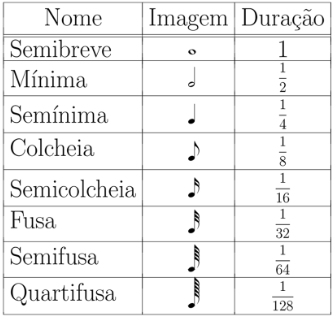
\includegraphics[width=3.125in,height=\textheight]{img/valores.png}

}

\subcaption{\label{fig-valores}Notas musicais e seus valores rítmicos}

\end{minipage}%
\newline
\begin{minipage}{\linewidth}

\centering{

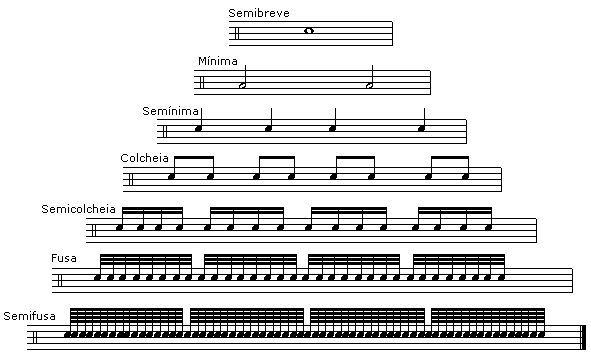
\includegraphics[width=4.16667in,height=\textheight]{img/hierarquia.png}

}

\subcaption{\label{fig-hierarquia}Relação hierárquica entre as notas
musicais}

\end{minipage}%

\caption{\label{fig-notas}Notas musicais e suas relações hierárquicas de
duração.}

\end{figure}%

A fração de compasso (Figura~\ref{fig-fração}) é a responsável por
indicar a quantidade de tempos que cada compasso possui, e a unidade de
tempo que será utilizada para contar esses tempos. O numerador da fração
indica a quantidade de tempos que cabem e cada compasso, enquanto o
denominador indica a unidade de tempo que será utilizada para contar
esses tempos. Por exemplo, uma fração de compasso \(4/4\) indica que
cada compasso possui \(4\) tempos, e que a unidade de tempo é a semínima
(\(1/4\)).

\begin{figure}

\centering{

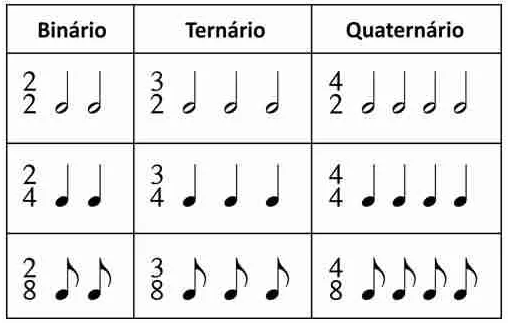
\includegraphics[width=3.125in,height=\textheight]{img/fração.png}

}

\caption{\label{fig-fração}Exemplos de frações de compasso}

\end{figure}%

Então, se um compasso tiver fração \(3/4\), isso significa que ele terá
3 tempos, e que a unidade de tempo é a semínima. Esse compasso pode
conter, por exemplo, três semínimas ou uma mínima e uma semínima
(Figura~\ref{fig-fração-2}).

\begin{figure}

\centering{

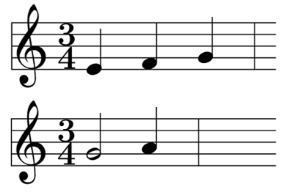
\includegraphics[width=3.125in,height=\textheight]{img/fração_2.png}

}

\caption{\label{fig-fração-2}Exemplos de compassos \(3/4\)}

\end{figure}%

Fica evidente que a teoria musical conta com conceitos e notação
matemática, de forma que a escolha da música como vetor para a
integração com a arte se mostra vantajosa para o ensino de frações, sem
qualquer necessidade de extrapolação de contexto --- a matemática já
está lá.

A equivalência se dá diretamente:

\begin{equation}\phantomsection\label{eq-fracao}{
\begin{aligned}
  \text{1 inteiro} &= \frac{1}{4} + \frac{1}{4} + \frac{1}{4} + \frac{1}{4} \\
 \musWhole &= \musQuarter + \musQuarter + \musQuarter + \musQuarter
\end{aligned}
}\end{equation}

\chapter{METODOLOGIA}\label{metodologia}

A atividade proposta consiste na exploração de conceitos de frações e
equivalência a partir das figuras rítmicas e fórmulas de compasso da
música
\href{https://open.spotify.com/intl-pt/track/2sUhjzuc6w4SRFwoC3LvXZ?si=594a3325c9c24baa}{Acorda
Pedrinho de Jovem Dionisio}. Essa música foi escolhida por dois
critérios. Primeiramente, como listado por SOUTO (2010), o tema deve ser
algo conhecido dos alunos, e essa música alcançou grande popularidade
entre as crianças brasileiras em plataformas de streaming entre 2022 e
2023. Em segundo lugar, a música possui uma melodia simples e muito
marcada, quase rítmica, o que facilita a identificação das figuras
rítmicas.

A atividade é composta por

\chapter{CONCLUSÃO}\label{conclusuxe3o}

\chapter*{REFERÊNCIAS}\label{referuxeancias}
\addcontentsline{toc}{chapter}{REFERÊNCIAS}

\phantomsection\label{refs}
\begin{CSLReferences}{0}{1}
\bibitem[\citeproctext]{ref-bresler_subservient_1995}
BRESLER, L. \href{https://doi.org/10.1080/10632913.1995.9934564}{The
Subservient, Co-Equal, Affective, and Social Integration Styles and
their Implications for the Arts}. \textbf{Arts Education Policy Review},
v. 96, n. 5, p. 31--37, 1 jun. 1995.

\bibitem[\citeproctext]{ref-frigotto_trabalho_2012}
FRIGOTTO, G.; CIAVATTA, M. Trabalho como Princípio Educativo. Em:
\textbf{Dicionário da Educação do Campo}. {[}s.l.{]} Epsjv - Fiocruz,
2012. p. 750--757.

\bibitem[\citeproctext]{ref-lovemore_enriching_2021}
LOVEMORE, T.; ROBERTSON, S.-A.; GRAVEN, M.
\href{https://doi.org/10.4102/sajce.v11i1.899}{Enriching the teaching of
fractions through integrating mathematics and music}. \textbf{South
African Journal of Childhood Education}, v. 11, 21 jan. 2021.

\bibitem[\citeproctext]{ref-maciel_educacao_2015}
MACIEL, C. L. A.
\href{https://doi.org/10.20500/rce.v10i20.2220}{{EDUCAÇÃO} {INTEGRAL}:
{LIMITES} E {POSSIBILIDADES} {SOB} A {HEGEMONIA} {DO} {CAPITAL}}.
\textbf{Revista Contemporânea de Educação}, v. 10, n. 20, p. 405 a
426--405 a 426, 17 dez. 2015.

\bibitem[\citeproctext]{ref-mello_tendencias_2007}
MELLO, A. C. C. D. \textbf{Tendências Em Educação Matemática}.
{[}s.l.{]} Unisulvirtual, 2007.

\bibitem[\citeproctext]{ref-robinson_arts_2013}
ROBINSON, A. H. \href{https://doi.org/10.1080/10632913.2013.826050}{Arts
Integration and the Success of Disadvantaged Students: A Research
Evaluation}. \textbf{Arts Education Policy Review}, v. 114, n. 4, p.
191--204, 1 out. 2013.

\bibitem[\citeproctext]{ref-souto_interdisciplinaridade_2010}
SOUTO, D. L. P. Interdisciplinaridade e aprendizagem da Matemática em
sala de aula, de Vanessa Sena Tomaz e Maria Manuela Martins Soares
David.(Coleção Tendências em Educação Matemática)--Belo Horizonte:
Autêntica, 2008. \textbf{Bolema-Boletim de Educação Matemática}, v. 23,
n. 36, p. 801--808, 2010.

\end{CSLReferences}



\end{document}
